\section{Sicurezza delle reti}

\subsection{Definizione e ambito della cybersecurity}

Nel moderno ecosistema digitale, la cybersecurity non è semplicemente un insieme
di strumenti tecnici, ma una dottrina sistematica volta alla protezione
dell'informazione in ogni sua forma: archiviata, trasmessa o elaborata. Tale
protezione si estende attraverso sistemi interconnessi, infrastrutture di rete
e linee di trasmissione, comprendendo l'intera architettura di Internet. La sua
rilevanza strategica risiede nella capacità di coniugare politiche organizzative
e misure tecniche per mitigare i rischi in un panorama globale sempre più ostile.

Per operare con rigore scientifico è necessario distinguere due domini fondamentali:

\begin{itemize}
\item \textbf{Information Security (sicurezza dell'informazione)}: si focalizza
sulla preservazione della triade CIA: Confidentiality (riservatezza), Integrity
(integrità), Availability (disponibilità). Include proprietà estese quali
l'autenticità e l'affidabilità dei dati.
\item \textbf{Network Security (sicurezza delle reti)}: è orientata alla
protezione delle infrastrutture e dei servizi da modifiche non autorizzate,
distruzione o divulgazione illecita. Il suo obiettivo primario è garantire che
la rete eroghi le proprie funzioni critiche in modo corretto, eliminando effetti
collaterali dannosi per l'integrità del sistema.
\end{itemize}

\subsection{Obiettivi della sicurezza: la triade CIA e requisiti estesi}

Il riferimento fondamentale per la categorizzazione degli obiettivi di sicurezza
è lo standard \textbf{NIST FIPS 199}, che definisce i requisiti e l'impatto della
perdita di sicurezza per ciascuna categoria.

\subsubsection{La triade CIA}

\paragraph{1) Riservatezza (Confidentiality)}

Garantisce la presenza di restrizioni autorizzate all'accesso o alla divulgazione
delle informazioni. Si distingue in:
\begin{itemize}
\item \textbf{Riservatezza dei dati}: garantisce che informazioni private o
proprietarie non siano rese accessibili a individui non autorizzati.
\item \textbf{Privacy}: assicura che gli utenti mantengano il controllo su quali
informazioni possono essere raccolte e a chi possano essere divulgate.
\end{itemize}

\paragraph{2) Integrità (Integrity)}

Protegge contro la modifica o la distruzione impropria delle informazioni. Si
articola in:
\begin{itemize}
\item \textbf{Integrità dei dati}: garantisce che dati e programmi siano
modificati solo secondo modalità autorizzate. Include l'Autenticità (l'oggetto
è effettivamente ciò che dichiara di essere) e il \textit{Non-Repudiation}
(non ripudio), che fornisce prova dell'invio o ricezione impedendo a una parte
di negare l'elaborazione di una transazione.
\item \textbf{Integrità del sistema}: assicura che il sistema svolga le sue
funzioni in modo ineccepibile, privo di manipolazioni deliberate o accidentali
delle sue componenti logiche o fisiche.
\end{itemize}

\paragraph{3) Disponibilità (Availability)}

Garantisce un accesso tempestivo e affidabile alle informazioni e ai servizi
per gli utenti autorizzati.

\subsubsection{Requisiti estesi: autenticità e accountability}

Oltre alla triade classica, la sicurezza moderna poggia su due pilastri
aggiuntivi:

\begin{itemize}
\item \textbf{Autenticità (Authenticity)}: la proprietà di essere genuini e
verificabili. Implica la certezza dell'identità degli utenti e la fiducia nella
validità della sorgente di ogni input che giunge al sistema.
\item \textbf{Responsabilità (Accountability)}: genera il requisito che le
azioni di un'entità siano tracciate in modo univoco. È un pilastro fondamentale
poiché i sistemi ``perfettamente sicuri'' sono un'astrazione ideale: la
tracciabilità supporta non solo l'analisi forense e il recupero post-incidente,
ma funge anche da deterrente, facilita l'isolamento dei guasti e supporta
le azioni legali.
\end{itemize}

Concettualmente, l'architettura della sicurezza può essere rappresentata come
un pentagono in cui il nucleo centrale, ``Information and Network Security'', è
sostenuto dai cinque pilastri: Riservatezza, Integrità, Disponibilità, Autenticità
e Responsabilità.

\subsection{Sfide progettuali e natura conflittuale della sicurezza}

La sicurezza è un processo dinamico e contraddittorio, una continua ``battaglia
d'ingegno'' tra il progettista e l'attaccante. Quest'ultimo gode di un vantaggio
asimmetrico: per compromettere un sistema è sufficiente individuare una singola
debolezza, mentre il difensore deve teoricamente proteggere ogni possibile punto
d'accesso. Spesso gli attacchi più efficaci derivano da un pensiero laterale che
sfrutta debolezze inaspettate nei meccanismi di difesa invece di colpire la
logica principale.

\paragraph{Complessità algoritmica e gestione dei segreti}

Una sfida critica riguarda la gestione delle informazioni segrete (esempio: chiavi
crittografiche). La sicurezza non risiede solo nell'algoritmo, ma nella creazione,
distribuzione e protezione di tali segreti. Inoltre, se un meccanismo di sicurezza
richiede limiti temporali stringenti per la consegna dei messaggi, la presenza di
ritardi variabili e imprevedibili nella rete può rendere nullo lo sforzo di
protezione.

\paragraph{Il conflitto tra sicurezza e usabilità}

Esiste una tensione intrinseca tra rigore tecnico ed efficienza operativa. Molti
utenti e amministratori percepiscono le misure di sicurezza restrittive come un
impedimento alla produttività. Questo porta spesso a considerare la sicurezza come
un \textit{afterthought} (pensiero a posteriori), implementata solo dopo che il
design del sistema è completo, invece di essere integrata nativamente nel ciclo
di vita dello sviluppo.

\paragraph{Impatto economico}

Il mantenimento della sicurezza richiede il monitoraggio costante e investimenti
continui in \textbf{CAPEX} (hardware e software) e \textbf{OPEX} (formazione del
personale e gestione operativa). La percezione del beneficio è spesso nulla fino
a quando non si verifica una violazione critica, rendendo difficile giustificare
i costi in contesti orientati al breve termine.

\subsection{Tassonomia della sicurezza secondo lo standard OSI/ITU-T X.800}

Per gestire sistematicamente questa complessità, lo standard \textbf{ITU-T X.800}
definisce una nomenclatura rigorosa per distinguere le componenti della sicurezza:

\begin{enumerate}
\item \textbf{Security Attack (attacco alla sicurezza)}: qualsiasi azione che
comprometta la sicurezza delle informazioni o dell'infrastruttura di
un'organizzazione. Si distingue tra \textbf{Minaccia (Threat)}, ovvero il
rischio potenziale di un evento avverso, e \textbf{Attacco}, ovvero l'attività
malevola effettivamente commessa.
\item \textbf{Security Mechanism (meccanismo di sicurezza)}: un processo o un
dispositivo (esempio: algoritmi crittografici, controllo degli accessi)
progettato per rilevare, prevenire o recuperare da un attacco.
\item \textbf{Security Service (servizio di sicurezza)}: una capacità che
implementa le politiche di sicurezza. I servizi di sicurezza utilizzano uno o
più meccanismi per contrastare gli attacchi.
\end{enumerate}

\subsection{Classificazione degli attacchi: passivi e attivi}

Gli attacchi si dividono in due categorie basate sul loro impatto sulle risorse
del sistema.

\subsubsection{Attacchi passivi (eavesdropping e traffic analysis)}

L'obiettivo è l'intercettazione delle informazioni senza alterare le risorse.
L'attaccante si pone lateralmente alla linea di comunicazione, osservando il
passaggio dei dati in modo trasparente.

\begin{itemize}
\item \textbf{Rilascio dei contenuti}: lettura diretta di messaggi non protetti.
\item \textbf{Analisi del traffico}: osservazione di frequenza e lunghezza dei
messaggi per dedurre la natura della comunicazione.
\end{itemize}

Questi attacchi sono quasi impossibili da rilevare poichè non alterano i dati;
l'unica difesa efficace è  la prevenzione, tipicamente attraverso la cifratura.

\subsubsection{Attacchi attivi}

Comportano la modifica del flusso di dati o la creazione di falsi flussi.
L'attaccante interrompe il flusso normale per intervenire direttamente.

\begin{itemize}
\item \textbf{Masquerade}: un'entità con pochi privilegi finge di essere
un'altra per ottenere vantaggi non autorizzati.
\item \textbf{Replay}: cattura di un'unità dati e sua successiva ritrasmissione.
\item \textbf{Modifica dei messaggi}: alterazione, ritardo o riordino della
comunicazione legittima.
\item \textbf{Denial of Service (DoS)}: sovraccarico della rete o soppressione
dei messaggi verso un target specifico. La protezione assoluta è impraticabile;
l'enfasi si sposta quindi sulla rilevazione e sul recupero.
\end{itemize}

\begin{figure}[H]
\centering
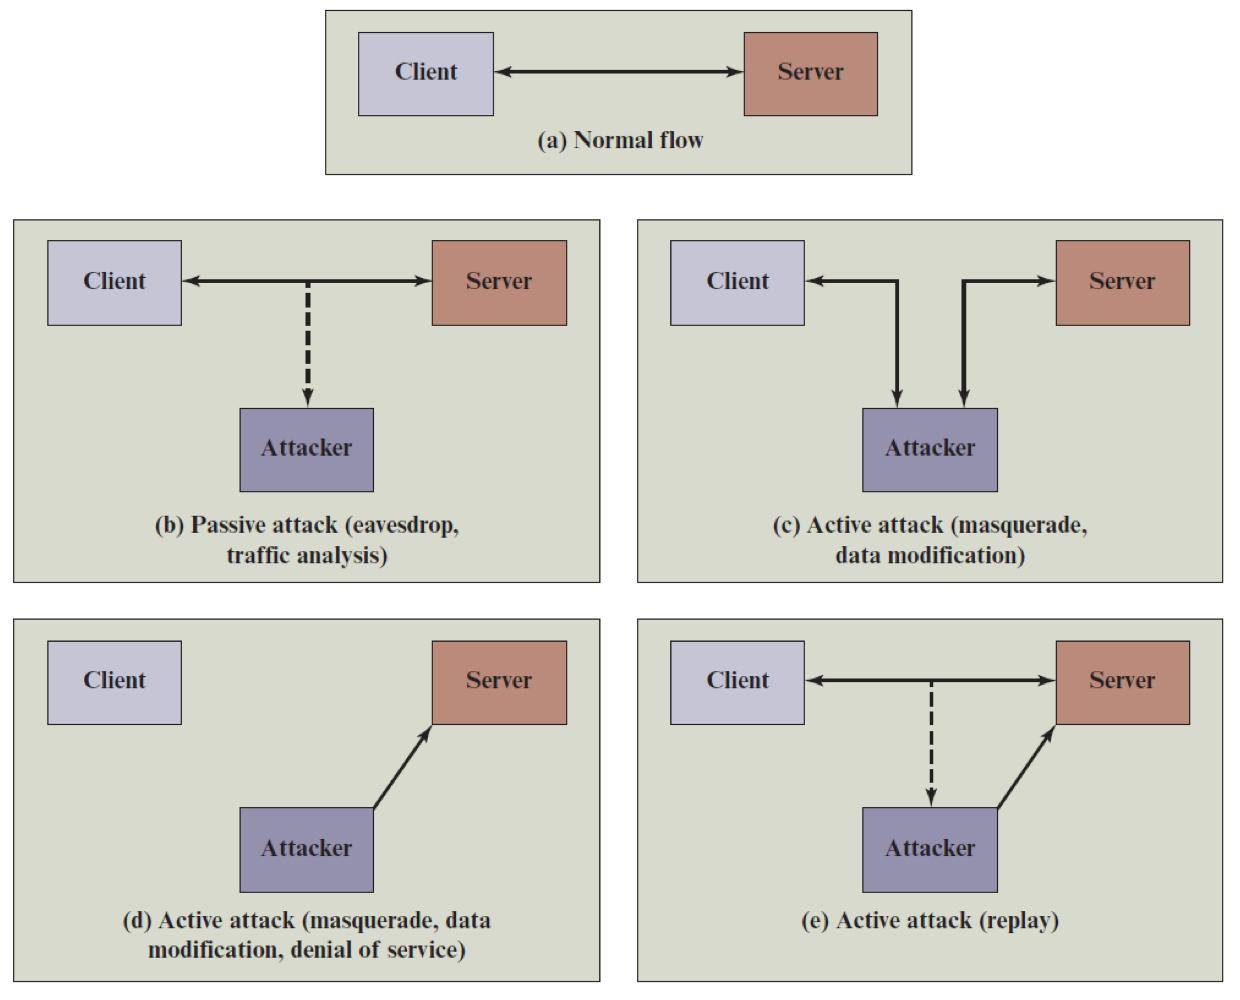
\includegraphics[width=0.6\textwidth]{img/attacks.png}
\end{figure}

\subsection{Servizi di sicurezza e protezione dei dati}

I servizi di sicurezza implementano le politiche organizzative per garantire i
requisiti CIA + AA:

\begin{itemize}
\item \textbf{Autenticazione}: assicura l'identità delle entità peer e l'origine
dei dati, prevenendo interferenze da terze parti (masquerade).
\item \textbf{Controllo degli accessi}: regola chi può accedere a quali risorse.
\item \textbf{Riservatezza dei dati}: protegge i dati dagli attacchi passivi,
applicabile a livello di intero host, singola sessione o singolo messaggio.
\item \textbf{Integrità dei dati}: si divide in \textbf{connectionless}
(protezione contro modifiche del singolo messaggio) e \textbf{connection-oriented},
che garantisce che il flusso arrivi senza duplicazioni, riordini o inserimenti,
coprendo anche la distruzione dei dati e il DoS.
\item \textbf{Non-Repudiation}: impedisce la negazione di trasmissione o ricevimento di un messaggio.
\end{itemize}

\subsection{Meccanismi tecnici e implementazioni}

I meccanismi sono i motori tecnologici che rendono operativi i servizi di
sicurezza. Tra i principali figurano:

\begin{itemize}
\item \textbf{Algoritmi crittografici}: reversibili per la cifratura o
irreversibili per l'hashing.
\item \textbf{Firme digitali}: per garantire autenticità e integrità, proteggendo
dalla falsificazione.
\item \textbf{Authentication Exchange}: processi tecnici per assicurare l'identità
dei peer.
\item \textbf{Access Control}: meccanismi per l'applicazione dei diritti di
accesso.
\item \textbf{Traffic Padding}: inserimento di dati artificiali per contrastare
l'analisi del traffico dell'attaccante.
\item \textbf{Controllo del routing}: selezione di percorsi sicuri e separati per diverse richieste di sicurezza.
\item \textbf{Notarizzazione}: garanzia di terze parti fidate sugli scambi.
\end{itemize}

\subsection{Architettura della sicurezza di rete: livelli e dispositivi}

La sicurezza deve essere distribuita strategicamente tra \textbf{Device Security}
(firewall e IDS/IPS per la protezione dei nodi) e \textbf{Communications Security}
(protocolli crittografici per i canali di comunicazione).

La stratificazione dello stack IP permette di scegliere il livello ottimale di
intervento:

\begin{itemize}
\item \textbf{Livello Network (IPsec)}: offre protezione a livello di indirizzo IP.
È il più trasparente per le applicazioni e gli utenti, proteggendo tutto il
traffico in modo uniforme.
\item \textbf{Livello Transport (SSL/TLS)}: fornisce sicurezza per protocolli come
HTTP o FTP. È specifico per le sessioni di trasporto e richiede che l'applicazione
sia consapevole della sua presenza.
\item \textbf{Livello Application (S/MIME, Kerberos)}: fornisce un controllo
granulare e specifico per l'applicazione (esempio: sicurezza end-to-end per la
posta elettronica). È la scelta ideale quando i requisiti di sicurezza sono legati
alla logica del servizio stesso.
\end{itemize}

\subsection{Analisi delle minacce a livello applicativo}

Nonostante le difese di rete, esistono minacce che colpiscono direttamente
l'utente finale. La tabella seguente riassume le principali dimensioni di rischio:

\begin{itemize}
\item \textbf{Integrità}: le minacce principali includono la modifica dei dati
dell'utente, la modifica della memoria, l'alterazione del traffico di messaggi in
transito e l'impiego di Trojan horse all'interno del browser. Gli effetti tipici
sono la perdita di informazioni, la compromissione della macchina e, soprattutto,
l'esposizione a ulteriori categorie di attacco. In questo contesto, una
contromisura fondamentale è l'uso di checksum crittografici per rilevare
alterazioni non autorizzate.
\item \textbf{Riservatezza}: rientrano in questa categoria l'eavesdropping sulla
rete, il furto di informazioni dal server o dal client e la raccolta indebita di
metadati, come la configurazione della rete o l'identità dei client che
comunicano con un server. Le conseguenze dirette sono la perdita di informazioni
e la compromissione della privacy. Le difese tipiche sono la cifratura dei dati
e l'uso di web proxy per limitare l'esposizione delle comunicazioni.
\item \textbf{Denial of Service}: gli attacchi possono manifestarsi tramite
terminazione dei thread utente, flooding della macchina con richieste fasulle,
esaurimento di disco o memoria oppure isolamento del sistema mediante attacchi
DNS. Le conseguenze sono di natura fortemente operativa: il servizio diventa
disruptive, l'utente subisce un degrado evidente dell'esperienza d'uso e, nei
casi peggiori, non riesce pi\`u a svolgere il proprio lavoro. Per loro natura,
questi attacchi risultano difficili da prevenire in modo assoluto.
\item \textbf{Autenticazione}: le minacce pi\`u rilevanti sono
l'impersonificazione di utenti legittimi e la falsificazione dei dati. Tali
attacchi producono una rappresentazione falsa dell'identit\`a dell'utente e
inducono il sistema o gli operatori a considerare valide informazioni che non
lo sono. La risposta pi\`u efficace consiste nell'adozione di tecniche
crittografiche per la verifica dell'identit\`a e della validit\`a dei dati.
\end{itemize}

Una protezione efficace non può prescindere da un approccio olistico che integri
gli obiettivi CIA+AA con meccanismi tecnici rigorosi, politiche chiare e
monitoraggio costante. Solo comprendendo la natura dinamica e conflittuale 
tra sicurezza e viabilità è possibile costruire sistemi efficienti nel tempo.

\begin{figure}[H]
\centering
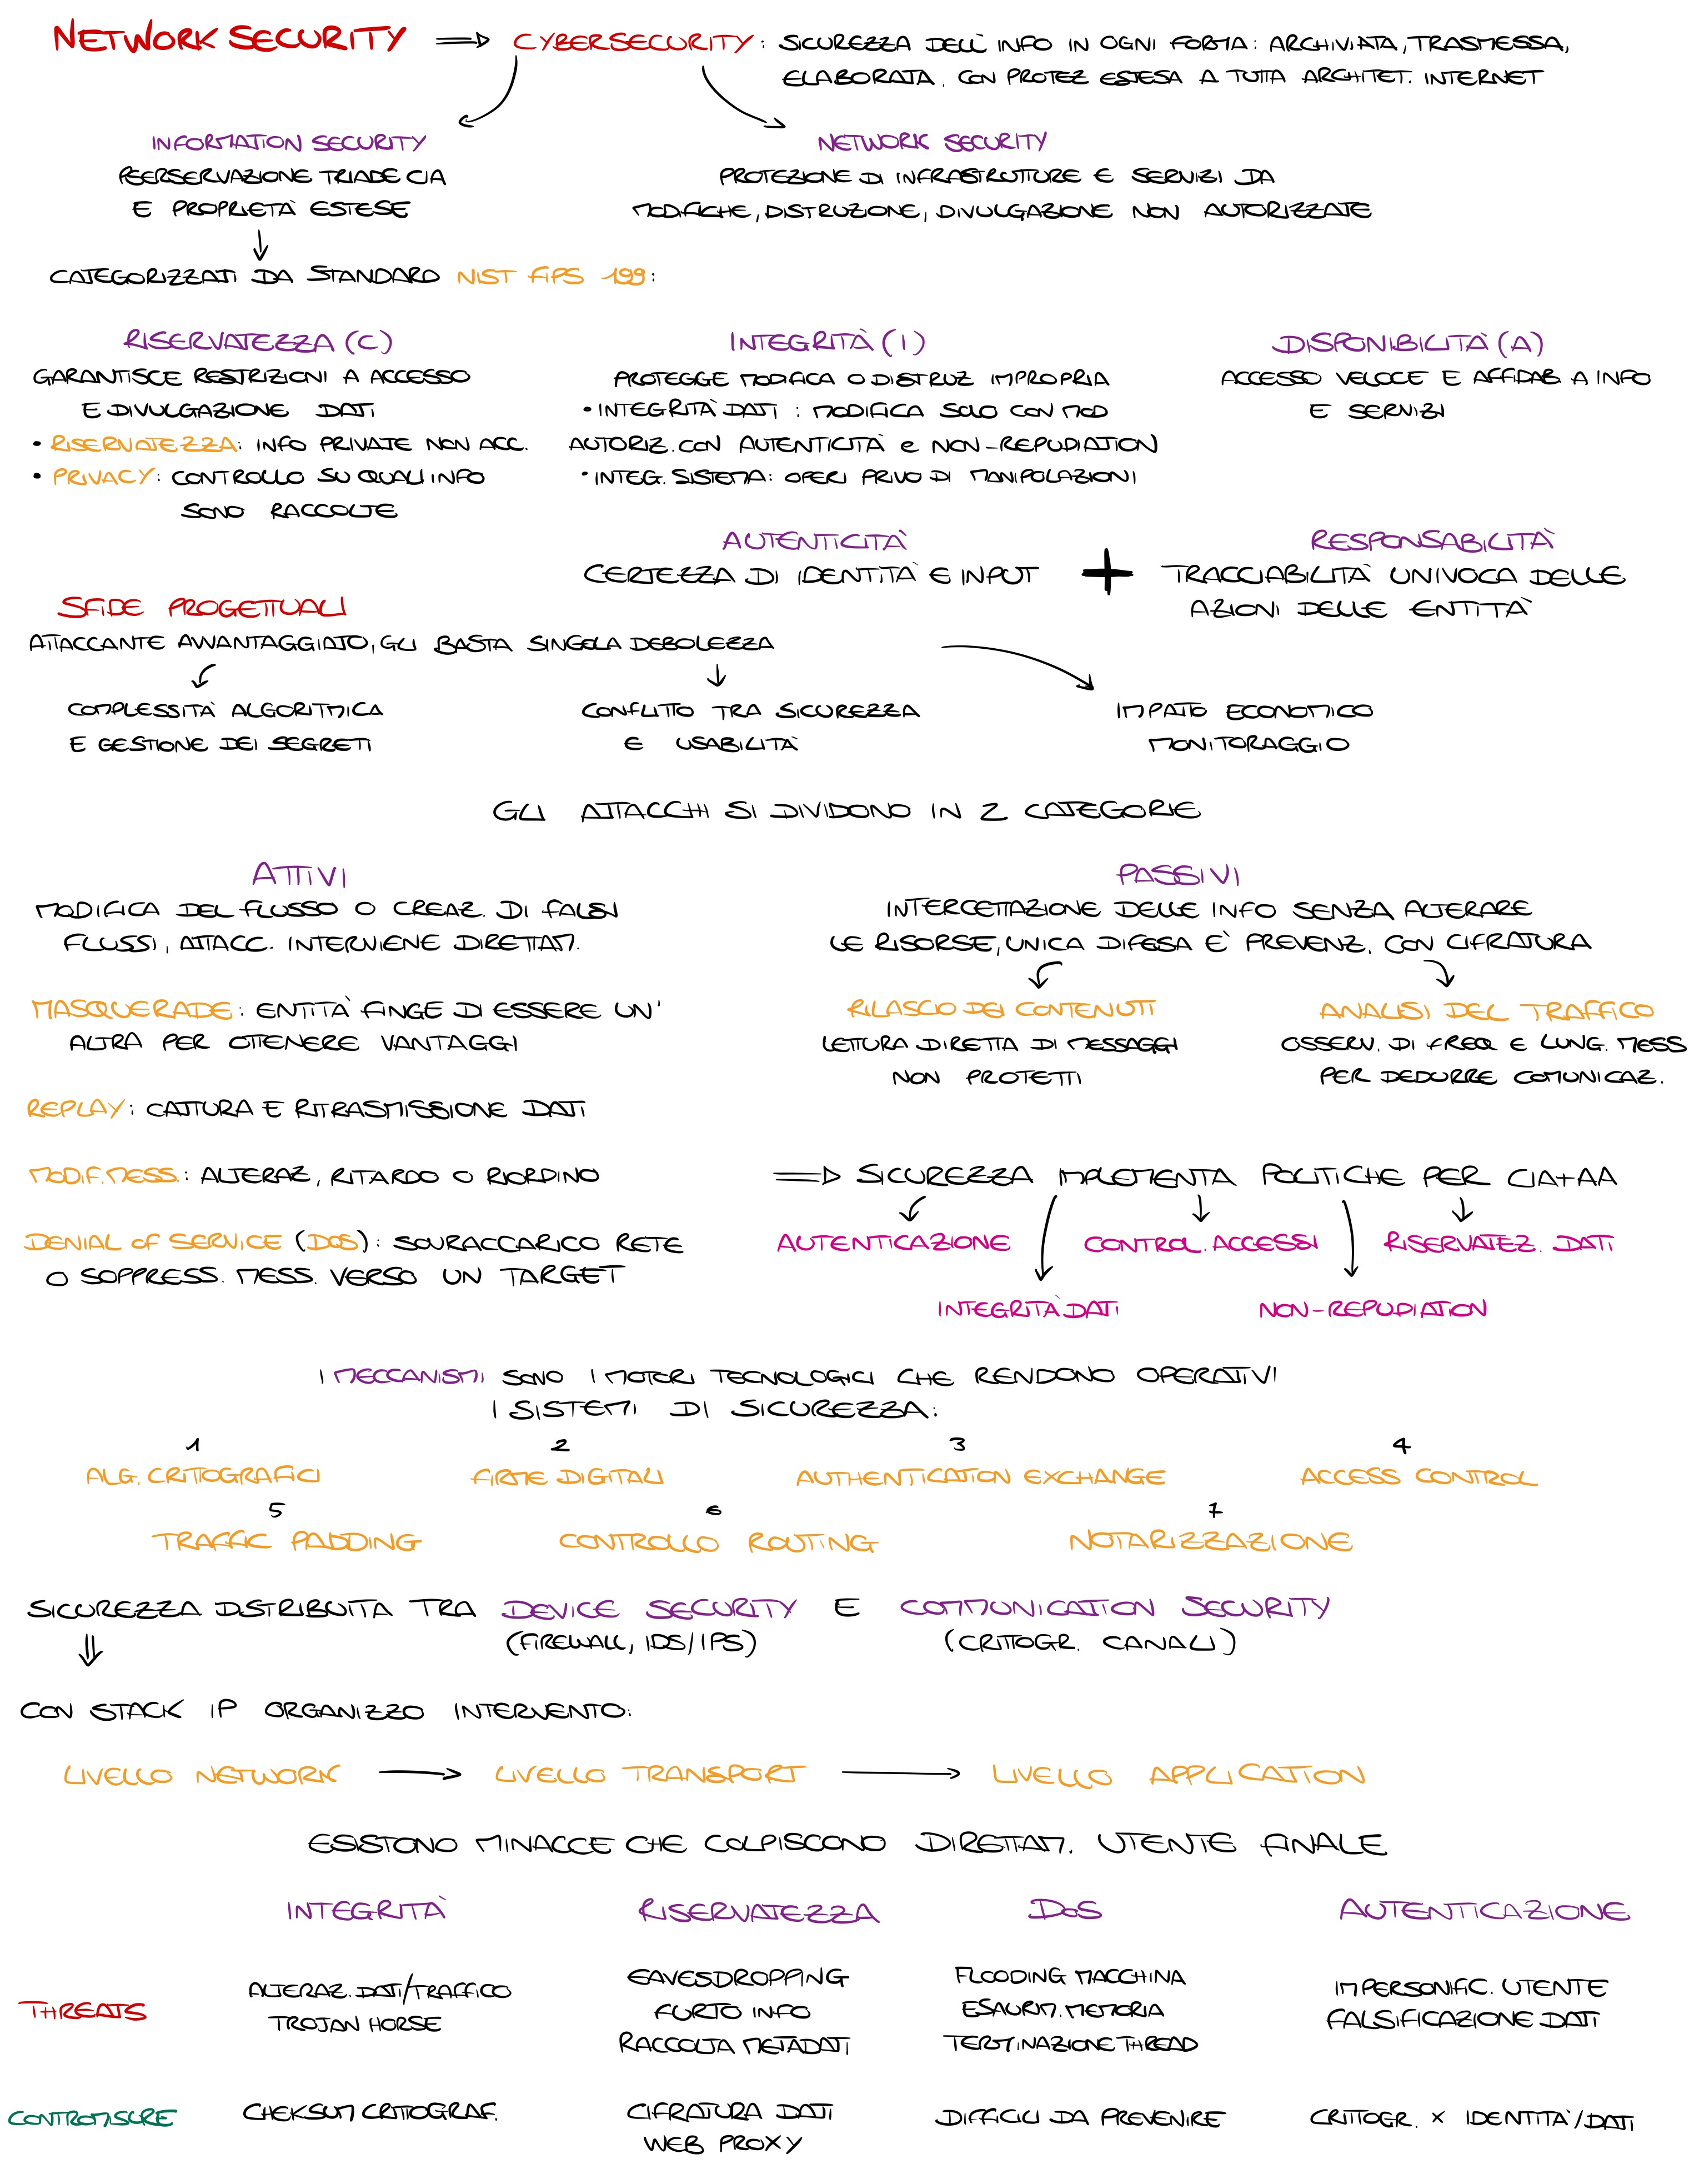
\includegraphics[width=1\textwidth]{img/3.jpg}
\end{figure}
